\documentclass[a4paper,11pt]{article}
\usepackage[a4paper, top=2.5cm, bottom=2.5cm, left=2cm, right=2cm]{geometry}

% --- 言語・フォント設定 (LuaLaTeX標準) ---
\usepackage{luatexja}
% フォントプリセットや個別のフォント設定は行わず、
% 環境のデフォルト（原ノ味フォント等）を使用します。

% --- パッケージ ---
\usepackage{amsmath}
\usepackage{amssymb}
\usepackage{amsthm}
\usepackage{mathrsfs}
\usepackage{tikz}
\usepackage{tikz-cd}
\usepackage{listings}
\usepackage{xcolor}

% --- TikZ設定 ---
\usetikzlibrary{arrows.meta, positioning, calc, shapes}

% --- コード掲載設定 ---
\lstset{
  basicstyle=\ttfamily\small,
  frame=single,
  breaklines=true,
  backgroundcolor=\color{gray!5},
  captionpos=b,
  language=bash, % Leanに近いハイライト用
  numbers=left,
  numberstyle=\tiny\color{gray},
  keywordstyle=\color{blue},
  commentstyle=\color{green!60!black}
}

% --- 定理環境 ---
\theoremstyle{definition}
\newtheorem{definition}{定義}[section]
\newtheorem{example}[definition]{例}
\theoremstyle{plain}
\newtheorem{theorem}[definition]{定理}
\newtheorem{lemma}[definition]{補題}
\newtheorem{proposition}[definition]{命題}

% --- メタデータ ---
\title{構造塔理論における停止時間の解釈: \texttt{minLayer} と停止過程\\
\large \textit{Lean 4による確率論の形式化プロジェクト}}

\author{
  \textbf{Gemini (Google)} \\
  \small \textit{TeXファイル生成・図式作成・解説執筆}
  \and
  \textbf{CODEX (OpenAI)} \\
  \small \textit{Leanコード生成・形式化原案}
}
\date{\today}

\begin{document}

\maketitle

\begin{abstract}
本稿では、構造塔 (Structure Tower) の枠組みを用いて確率論における「停止時間 (Stopping Time)」を再解釈する手法について述べる。
特に、ある事象が可測となる最小の時刻を与える \texttt{minLayer} 演算子が、停止時間の概念と自然に対応することを示す。
また、停止 $\sigma$-代数や停止過程の構成について、Lean 4による実装コードを交えて解説する。
\end{abstract}

\tableofcontents

\section{はじめに}
確率論の形式化において、フィルトレーション $(\mathcal{F}_n)_{n \in \mathbb{N}}$ と停止時間 $\tau$ は中心的な役割を果たす。
構造塔理論の視点からは、フィルトレーションは $\sigma$-代数の階層構造であり、停止時間は「情報が確定する時刻」として捉えられる。

本稿で扱う \texttt{StoppingTime\_MinLayer.lean} は、以下の要素を提供する。
\begin{itemize}
    \item フィルトレーションを構造塔 \texttt{StructureTowerMin} へ変換する機構。
    \item 停止集合 $\{\tau \le n\}$ と構造塔の層 (Layer) との対応。
    \item 単一の標本点 $\omega$ が識別可能になる「最初の時刻」としての \texttt{minLayer}。
\end{itemize}

\section{フィルトレーションと構造塔の接続}

\subsection{構造塔への昇格}
フィルトレーション $\mathcal{F}$ は、各時刻 $n$ に $\sigma$-代数を対応させる単調写像である。
これを構造塔の言葉で記述すると、各 $n$ に対して「$\mathcal{F}_n$-可測な集合の族」を対応させる写像となる。

\begin{definition}[Tower of Filtration]
フィルトレーション $\mathcal{F}$ から誘導される構造塔 $T(\mathcal{F})$ は以下のように定義される。
\[ \mathrm{layer}(n) = \{ A \subseteq \Omega \mid A \in \mathcal{F}_n \} \]
\end{definition}

Leanコードでは以下のように実装されている。

\begin{lstlisting}[caption=フィルトレーションの構造塔化]
/-- フィルトレーションを構造塔に昇格する。 -/
noncomputable def towerOf (ℱ : Filtration Ω) :
    StructureTowerMin (Set Ω) ℕ :=
  SigmaAlgebraFiltrationWithCovers.FiltrationToTower (Ω := Ω) ℱ
\end{lstlisting}

\subsection{停止集合の所属}
停止時間 $\tau$ の定義条件 $\forall n, \{ \tau \le n \} \in \mathcal{F}_n$ は、構造塔の用語では「集合 $\{ \tau \le n \}$ が $n$ 番目の層に属する」と言い換えられる。

\begin{figure}[htbp]
\centering
\begin{tikzpicture}[x=1.5cm, y=1.2cm]
    % Time axis
    \draw[->, thick] (0,0) -- (5,0) node[right] {時刻 $n$};
    
    % Layers
    \foreach \x in {1, 2, 3, 4} {
        \draw (\x, 0.1) -- (\x, -0.1) node[below] {$\x$};
        \node[draw, ellipse, minimum width=1.2cm, minimum height=0.8cm, fill=blue!10] (L\x) at (\x, 1.5) {$\mathcal{F}_{\x}$};
    }
    
    % Stopping Set intuition
    \node[align=center] at (2.5, 3) {停止集合 $\{\tau \le n\}$ \\ は $\mathcal{F}_n$ の要素};
    \draw[->, dashed] (2.5, 2.7) -- (L2);
    \draw[->, dashed] (2.5, 2.7) -- (L3);
    
    % Inclusion
    \draw[->] (L1) -- (L2);
    \draw[->] (L2) -- (L3);
    \draw[->] (L3) -- (L4);
    
    \node at (0, 1.5) {情報の解像度};
\end{tikzpicture}
\caption{フィルトレーションの層と停止集合の関係}
\end{figure}

\section{\texttt{minLayer} と最初の可測時刻}

構造塔の \texttt{minLayer} 関数は、ある要素が初めて層に現れる添字を返す。
確率空間上の点 $\omega$ に対して、単集合 $\{\omega\}$ が初めて可測集合となる時刻は、その $\omega$ が他の点と完全に区別可能になる時刻と解釈できる。

\begin{definition}[First Measurable Time]
標本点 $\omega \in \Omega$ に対する「最初の可測時刻」を以下で定義する。
\[ \tau_{\omega} = \mathrm{minLayer}(\{\omega\}) = \min \{ n \in \mathbb{N} \mid \{\omega\} \in \mathcal{F}_n \} \]
\end{definition}

これは、情報が増えるにつれて $\omega$ の特定が可能になるプロセスを表している。

\begin{lstlisting}[caption=単点の最初の可測時刻]
/-- 単点 {ω} が初めて可測になる時刻。 -/
noncomputable def firstMeasurableTime (ℱ : Filtration Ω) (ω : Ω) : ℕ :=
  (towerOf (Ω := Ω) ℱ).minLayer {ω}
\end{lstlisting}

\begin{figure}[htbp]
\centering
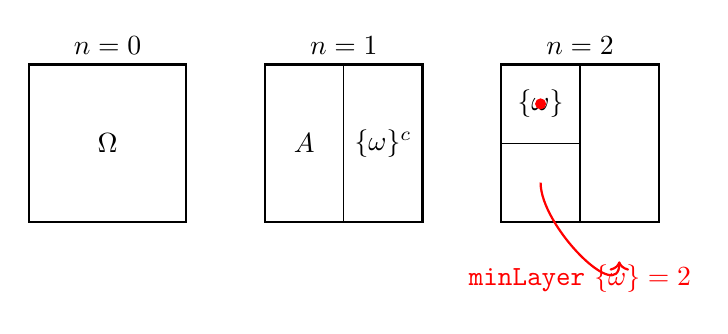
\begin{tikzpicture}
    % Conceptual diagram of partition refinement
    
    % Time 0: Coarse
    \draw[thick] (0,0) rectangle (2,2);
    \node at (1,1) {$\Omega$};
    \node[above] at (1,2) {$n=0$};
    
    % Time 1: Split
    \draw[thick] (3,0) rectangle (5,2);
    \draw (4,0) -- (4,2);
    \node at (3.5,1) {$A$};
    \node at (4.5,1) {$\{\omega\}^c$};
    \node[above] at (4,2) {$n=1$};
    
    % Time 2: Fine (omega isolated)
    \draw[thick] (6,0) rectangle (8,2);
    \draw (7,0) -- (7,2);
    \draw (6,1) -- (7,1);
    \node at (6.5, 1.5) {$\{\omega\}$}; % Here omega is isolated
    \fill[red] (6.5, 1.5) circle (2pt);
    \node[above] at (7,2) {$n=2$};
    
    \draw[->, thick, red] (6.5, 0.5) to[out=-90, in=-90] node[below] {\texttt{minLayer} $\{\omega\} = 2$} (7.5, -0.5);

\end{tikzpicture}
\caption{情報の細分化と単点の分離（可測化）。時刻 $n=2$ で初めて $\{\omega\}$ が $\sigma$-代数の元となり、分離される様子。}
\end{figure}

\section{停止過程とオプショナル停止}

停止時間 $\tau$ を用いて確率過程 $X_n$ を止める操作は、マルチンゲール理論において重要である。
本形式化では、停止過程 \texttt{stopped} を純粋な関数として定義し、その後に測度論的な性質（可測性・可積分性）を付与するアプローチをとっている。

\begin{definition}[Stopped Process]
過程 $X$ と停止時間 $\tau$ に対し、停止過程 $X^\tau$ を以下で定義する。
\[ X^\tau_n(\omega) = X_{n \land \tau(\omega)}(\omega) \]
\end{definition}

\begin{figure}[htbp]
\centering
\begin{tikzpicture}[domain=0:5, scale=1.2]
    % Axes
    \draw[->] (-0.2,0) -- (5.5,0) node[right] {$n$};
    \draw[->] (0,-0.5) -- (0,3) node[above] {$X_n(\omega)$};
    
    % Original Process (dashed)
    \draw[gray, dashed] plot[mark=x] coordinates {(0,0) (1,1) (2,1.5) (3,2.5) (4,2) (5,3)};
    \node[gray] at (5,3.2) {$X_n$};
    
    % Stopping Time tau(omega) = 2
    \draw[red, thick] (2,0) -- (2,3);
    \node[red, below] at (2,0) {$\tau(\omega)=2$};
    
    % Stopped Process (blue solid)
    \draw[blue, thick] plot[mark=*] coordinates {(0,0) (1,1) (2,1.5)};
    \draw[blue, thick] (2,1.5) -- (5,1.5);
    \foreach \x in {3,4,5} \draw[blue, fill=blue] (\x, 1.5) circle (1.5pt);
    
    \node[blue] at (4, 1.7) {$X^\tau_n$ (固定)};

\end{tikzpicture}
\caption{停止過程の挙動。$\tau(\omega)$ 以降、値は $X_{\tau(\omega)}$ に固定される。}
\end{figure}

Leanコードでは、`Nat.min` を用いて簡潔に表現されている。

\begin{lstlisting}[caption=停止過程の定義]
/-- 停止過程（純粋に関数レベルの定義）。 -/
def stopped {β : Type*} (X : ℕ → Ω → β) (τ : Ω → ℕ) :
    ℕ → Ω → β :=
  fun n ω => X (Nat.min n (τ ω)) ω
\end{lstlisting}

\section{結論と今後の展望}
構造塔の視点を導入することで、確率論における「情報の増大」と「可測性」の関係が、順序集合上の層構造として明確に記述された。
特に、\texttt{minLayer} による停止時間の定式化は、計算機科学的な「探索」の概念と確率論的な「待機時間」の概念を結びつける興味深い視点を提供している。

今後は、この基盤の上にオプショナル停止定理やマルチンゲールの収束定理を形式化していくことが目標となる。

\end{document}